% !TEX encoding = UTF-8 Unicode
\documentclass[12pt,a4paper]{report}

\usepackage[brazil]{babel}
\usepackage[utf8]{inputenc}
\usepackage[T1]{fontenc}
\usepackage{graphicx, subfigure}
\usepackage{indentfirst}
\usepackage{color}

\graphicspath{ {images/} }

\title{Análise de redes de comunicação através de \textit{packet sniffing}}
\author{Alexandre Lucchesi Alencar\\
	09/0104471\\
	alexandre@loopec.com.br
	\and
	Pedro Salum Franco\\
	09/0139232\\
	pedro@loopec.com.br
	\and
	Daniel A. M. Sandoval\\
	09/0109899\\
	daniel@loopec.com.br}
\begin{document}
\maketitle

\begin{abstract}
O presente trabalho 
%resumo do relatório que deve conter objetivo do experimento, resultados chaves, pontos maiores de discussão, resultados mais importantes
\end{abstract}

\tableofcontents

\chapter{Introdução}
%introdução: background ou conceitos teóricos relacionados, descrição do equipamento utilizado, restrições no experimento
A transmissão de informação em redes como a Internet ou LANs se dá através da divisão da informação em pacotes, que são transmitidos nos mais diversos meios - Wi-Fi, Bluetooth, rádio, cabos de pares trançados, par metálico, fibra ótica - para chegar da origem ao seu destino.
Os protocolos de rede nas camadas física, enlace, rede, transporte e aplicação são responsáveis por tornar essa comunicação transparente e viável por todo o globo terrestre.

O presente projeto tem como objetivo a análise de redes de comunicação através da técnica conhecida como \textit{packet sniffing}, ou seja, examinar os pacotes que são enviados e recebidos para análise da eficiência da rede de comunicação sendo utilizada.

\section{Fundamentação Teórica}

\paragraph{\textit{Packet sniffing}} Técnica que consiste na análise dos pacotes que trafegam na rede, sejam eles endereçados à estação que está monitorando ou não. Através dessa técnica é possível medir a eficiência e taxa de ocupação de uma rede, além de interceptar toda o conteúdo de comunicação não criptografada.

\paragraph{Roteador} Dispositivo capaz de interligar duas redes realizando tradução de endereços, permitindo a criação de redes cada vez maiores.

\paragraph{\textit{Hops}} Os pacotes transmitidos podem trafegar entre diversas redes para chegar ao seu destino. Quando o pacote passa de uma rede para outra através de um roteador, chamamos isso de \textit{hop}.

\paragraph{\textit{Handshaking}} Processo onde ocorre troca de pacotes entre duas estações com o objetivo de se estabelecer uma conexão.

\paragraph{\textit{Ping}} Ferramenta que testa a conexão entre duas estações. Muito utilizada para medir performance, através do tempo que leva para a estação que ``pinga'' outra estação receber uma resposta, ou ``\textit{pong}''.

\section{Equipamentos Utilizados}

Para atingir os objetivos desse projeto, utilizamos os seguintes equipamentos e ferramentas:

\begin{description}
\item[MacBook Air] Como estação de \textit{packet sniffing}, utilizamos um MacBook Air de 13'' com 4GB de memória RAM e processador Intel Core i7 1.8GHz;
\item[Wireshark] Para poder capturar os pacotes, utilizamos o software Wireshark, que é \textit{open-source} e funciona monitorando atividade na interface de rede e capturando todos os pacotes que chegam a ela;
\item[AirPort Express] Para a criação da rede à qual foi conectado o MacBook, foi utilizado um AirPort Express configurado para criar uma rede WiFi no padrão \(802.11g\), a uma taxa de \(54Mbps\);
\item[D-Link DI-634M] Roteador utilizado para criação de uma subrede para compartilhamento do IP único de saída;
\item[www.ip-address.com] Ferramenta utilizada para estimativa da distância física em quilômetros entre a estação de teste e os sites escolhidos para teste.
\end{description}

A fim de realizar os testes necessários, foram utilizadas as seguintes conexões com a Internet:

\begin{description}
\item[CDT/UnB] Conexão direta ao \textit{backbone} das Universidades brasileiras, através de um endereço IP fixo fornecido pelo Centro de Apoio ao Desenvolvimento Tecnológico da Universidade de Brasília (CDT/UnB);
\item[Oi] Conexão ADSL à Internet com taxa de transferência contratada de \(2Mbps\) fornecida pela empresa OI S.A.
\end{description}

\chapter{Parte I}

\paragraph{Objetivo} A Parte I tem como objetivo a medição e análise de aspectos do tráfego de rede. Através da análise dos tempos de resposta a \textit{ping} e de \textit{handshaking} da conexão TCP, pretendemos traçar relação entre a distância física e número de \textit{hops} entre os pontos da rede e os tempos medidos.

\section{\textit{Handshaking} TCP}

\subsection{Procedimento Experimental}

\paragraph{Definição dos casos de teste} Foram escolhidos quatro sites da Internet de acordo com a distância física com a estação de teste, com o objetivo de observar as variações de acordo com a distância até o destino. A relação de sites escolhidos para o teste está representada na Tabela~\ref{tab:siteshandshaking}, bem como o número de \textit{hops} e distância física em quilômetros até o servidor.

\begin{table}[h]
	\center
	\begin{tabular}{l*{6}{c}r}
	Site						& Hops	& Distância (km)	& Localização\\
	\hline
	www.bangladesh.gov.bd		& 24		& 15.465,6		& Bangladesh\\
	www.thepiratebay.se		& 15		& 10.180,8		& Suécia\\
	www.km.gov.al				& 15		& 9.363,2			& Albânia\\
	www.cic.unb.br				& 6		& 5				& Brasil\\
	\end{tabular}
	\caption{Sites escolhidos para teste de \textit{handshaking} TCP}
	\label{tab:siteshandshaking}
\end{table}

\paragraph{Escolha da conexão de rede} Para a realização dos testes foi escolhida a rede do CDT/UnB, com o objetivo de verificarmos resultados mais interessantes, principalmente pelo site www.cic.unb.br estar hospedado na mesma infraestrutura e pela qualidade da conexão.

\paragraph{Preparo do ambiente de testes} Com o objetivo de aproximar os testes de um caso real de uma rede de alto tráfego, durante os testes outras estações estavam utilizando a mesma conexão para \textit{streaming} de vídeo e videoconferência via Skype.

\paragraph{Medição dos tempos de \textit{handshaking}} Através da utilização da ferramenta Wireshark, medimos o tempo decorrido entre o envio do primeiro pacote TCP ao site e o recebimento de sua resposta. Um exemplo da visualização fornecida pela ferramenta para os pacotes enviados e recebidos está representada pela Figura~\ref{fig:wirebangladesh}. Os tempos medidos foram armazenados em arquivos de texto para análise posterior.

\begin{figure}[h]
\centering
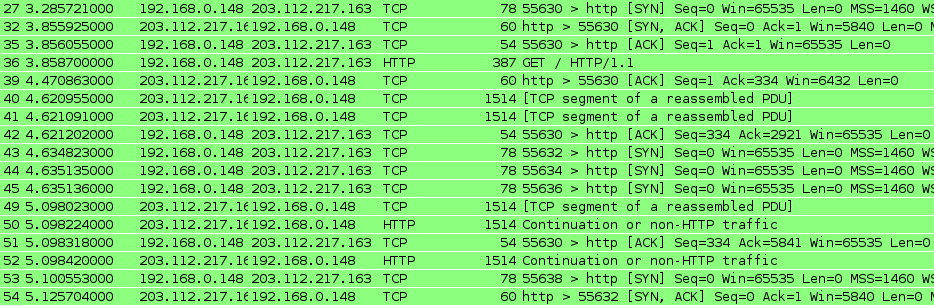
\includegraphics[width=\textwidth]{bangladesh.png}
\caption{\textit{Packet sniffing} da conexão com o site www.bangladesh.gov.bd}
\label{fig:wirebangladesh}
\end{figure}

\subsection{Resultados e Análise}

Os resultados obtidos foram de acordo com o esperado. Quanto maior a distância física e número de \textit{hops} entre a estação de teste e o site sendo testado, maior o tempo para completar o \textit{handshake}, (\(T_{hs}\)), conforme mostrado na Tabela~\ref{tab:resultshandshaking}.

\begin{table}[h]
	\center
	\begin{tabular}{l*{6}{c}r}
	Site						& Hops	& Distância (km)	& \(T_{hs} (ms)\)\\
	\hline
	www.bangladesh.gov.bd		& 24		& 15.465,6		& 570,204\\
	www.thepiratebay.se		& 15		& 10.180,8		& 314,048\\
	www.km.gov.al				& 15		& 9.363,2			& 306,378\\
	www.cic.unb.br				& 6		& 5				& 7,723\\
	\end{tabular}
	\caption{Tabela compilada dos resultados obtidos no teste de \textit{handshaking}}
	\label{tab:resultshandshaking}
\end{table}

\subsubsection*{Análise}

Apesar de haver uma relação clara entre a distância física, número de \textit{hops} e \(T_{hs}\), não é possível generalizar ou sequer traçar uma relação matemática. Percebe-se que \(T_{hs}\) depende da qualidade da conexão em geral, que é afetada pela distância, porém não exclusivamente.

Para conexão com o site www.cic.unb.br, percebemos que \(T_{hs}\) é muito reduzido, o que atribuímos a estar na mesma infraestrutura de rede que a estação de teste. Em comparação, a conexão com o site localizado em Bangladesh, a mais de 15 mil quilômetros de distância, \(T_{hs}\) é 7200\% maior.

Conforme esperado, a relação entre distância, número de \textit{hops} e o tempo para \textit{handshaking} não é direta porém está presente. Em geral, quanto maior a distância, maior o número de \textit{hops} e maior o tempo necessário para se estabelecer uma conexão.

\section{\textit{Ping}}

\subsection{Procedimento Experimental}

\paragraph{Definição dos casos de teste} Os sites escolhidos para os testes de \textit{ping} foram inicialmente os mesmos utilizados para testes de \textit{handshaking}. Porém, os sites www.thepiratebay.se e www.km.gov.al não responderam a \textit{pings}. Portanto, os retiramos do teste e adicionamos os sites www.google.com e www.terra.com.br. Os sites escolhidos estão listados na Tabela~\ref{tab:sitesping}, bem como o respectivo número de \textit{hops} e distância física em quilômetros até o servidor.

\begin{table}[h]
	\center
	\begin{tabular}{l*{6}{c}r}
	Site						& Hops	& Distância (km)	& Localização\\
	\hline
	www.bangladesh.gov.bd		& 24		& 15.465,6		& Bangladesh\\
	www.google.com		& 7		& 9.684,8		& EUA\\
	www.terra.com.br				& 5		& 996,8			& Brasil\\
	www.cic.unb.br				& 6		& 5				& Brasil\\
	\end{tabular}
	\caption{Sites escolhidos para teste de \textit{ping}}
	\label{tab:sitesping}
\end{table}

\paragraph{Escolha da conexão de rede} Para a realização dos testes foi escolhida a rede fornecida pela OI S.A., devido ao bloqueio implementado pela rede CDT/UnB a \textit{pings}. Porém, para o caso específico do site www.cic.unb.br, utilizamos a rede do CDT/UnB por serem permitidos \textit{pings} que não cruzam a fronteira da rede da UnB.

\paragraph{Preparo do ambiente de testes} Com o objetivo de aproximar os testes de um caso real de uma rede de alto tráfego, os testes foram realizados sob a mesmo cenário dos testes de \textit{handshaking}, com outras estações utilizando a mesma conexão para \textit{streaming} de vídeo e videoconferência via Skype.

\paragraph{Medição dos tempos de \textit{ping}} Através da utilização da ferramenta Ping, do próprio sistema operacional Mac OS X, efetuamos o teste de \textit{ping} para cada site separadamente. Cada teste foi realizado cinco vezes e o tempo considerado foi o médio constatado. Os tempos medidos foram armazenados em arquivos de texto para análise posterior.

\subsection{Resultados e Análise}

Os resultados obtidos foram de acordo com o esperado. Quanto maior a distância física e número de \textit{hops} entre a estação de teste e o site sendo testado, maior o tempo para completar o \textit{ping}, (\(T_{ping}\)), conforme mostrado na Tabela~\ref{tab:resultsping}.

\begin{table}[h]
	\center
	\begin{tabular}{l*{6}{c}r}
	Site						& Hops	& Distância (km)	& \(T_{ping}\)(ms)\\
	\hline
	www.bangladesh.gov.bd		& 24		& 15.465,6		& 523,186\\
	www.google.com		& 7		& 9.684,8		& 181,996\\
	www.terra.com.br				& 5		& 996,8			& 58,081\\
	www.cic.unb.br				& 6		& 5				& 2,519\\
	\end{tabular}
	\caption{Resultados obtidos para teste de \textit{ping}}
	\label{tab:resultsping}
\end{table}

\subsubsection*{Análise}

Os resultados foram muito similares aos obtidos nos testes de \textit{handshaking}, conforme esperado. Ainda em comparação com o teste de \textit{handshaking}, destaca-se a diferença \(T_{hs} - T_{ping} = 5,204 ms\), o que representa tempo de \textit{handshaking} 206\% maior do que o tempo de \textit{ping}. Resultado interessante quando comparado ao ocorrido para o site www.bangladesh.gov.bd, para o qual a mesma relação é de apenas 9\%. Esse resultado é esperado uma vez que pequenas variações serão muito mais significativas quando o próprio tempo é pequeno.

%Parte 1:
%Nesta parte, devem ser medidos alguns aspectos do tráfego de rede. Deve ser mostrada a figura da captura do pacote ou execução do comando que justifique a resposta da pergunta e de preferência plotagens de gráficos que ajudem na compreensão dos resultados.
%1.1 Enquanto Wireshark está funcionando, conectar a um site com o seu navegador. Quanto tempo leva para completar o handshaking necessário para estabelecer a conexão? Agora variar a distância para o site que você está se conectando. Isso muda o tempo de conexão? O tempo de conexão dependerá de outras coisas - como hora do dia, número de saltos, etc. Mostre um comparativo dos resultados, analisando os valores obtidos e os fatores que implicam na alteração dos valores obtidos. 1.2 Enquanto o Wireshark está em execução, pingar um número de sites e determinar o tempo exato necessário para que o ping (ver referências do comando ping no DOS e no Linux) seja completado. Quais são as variáveis que influenciam nos valores obtidos (distância, número de hops ? ).
%Parte 2:
%Acessar um site da sua escolha. Responda as perguntas a seguir, com base no conteúdo do quadro Ethernet contendo a mensagem HTTP GET. Ao responder a uma pergunta, deve ser mostrada a figura da captura do pacote que justifique a resposta da pergunta.
%2.1 Qual é o endereço de 48 bits Ethernet do seu computador?
%2.2 Qual é o endereço de destino de 48 bits no quadro Ethernet? É este o endereço Ethernet do site acessado (Dica: a resposta é não, mas você precisa justificar o motivo). Que dispositivo tem esse endereço Ethernet?
%2.3 Quantos bytes desde o início do quadro Ethernet faz o ASCII "G" em "GET" aparecem no quadro Ethernet?
%Responda às seguintes questões, com base no conteúdo do quadro de Ethernet que contém o primeiro byte da mensagem de resposta HTTP.
%2.4 Qual é o valor do endereço de origem Ethernet? É este o endereço do seu computador, ou do site acessado ?
%2.5 Qual é o endereço de destino no quadro Ethernet? É este o endereço Ethernet do seu computador?

%\chapter{Procedimento}
%Procedimento (descrição das ações realizadas, justificativa no caso de mudança de procedimento)

\chapter{Parte II}

\paragraph{Objetivo} A Parte II tem como objetivo a medição e análise de uma requisição HTTP GET.

\begin{figure}[h]
\centering
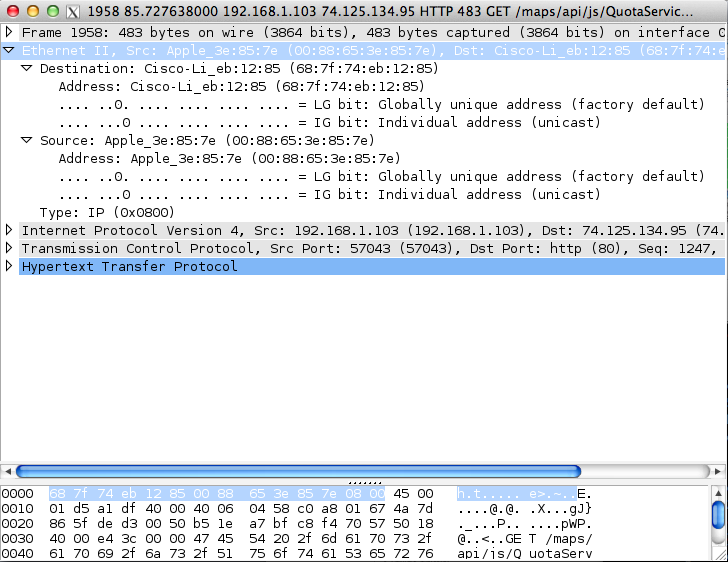
\includegraphics[width=\textwidth]{Ethernet-source-destination.png}
\caption{Origem e destino do pacote de rede}
\label{fig:ethernetsd}
\end{figure}

\paragraph{2.1} Endereço: 00:88:65:3e:85:7e.

\paragraph{2.2} Endereço: 68:7f:74:eb:12:85. Não, esse é o endereço do roteador conectado à rede local. O roteador é da Linksys (Cisco), como pode-se perceber na Figura~\ref{fig:ethernetsd} tem uma referência ao nome ``Cisco'' junto ao host destino.

\paragraph{2.3} Como se pode ver na Figura~\ref{fig:get}, antes do `G', tem-se 54 bytes. O caracter `G' de ``GET'' corresponde ao valor hexadecimal 0x47. Podemos observar na tabela ASCII que esse número é o correspondente ao ``G'' maiúsculo.

\begin{figure}[h]
\centering
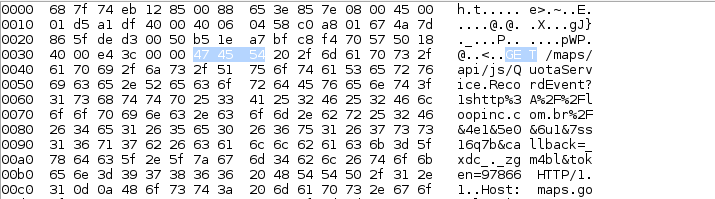
\includegraphics[width=\textwidth]{GET.png}
\caption{Conteúdo completo do pacote, em notação Hexadecimal e símbolo ASCII}
\label{fig:get}
\end{figure}

\paragraph{2.4} Endereço: 00:88:65:3e:85:7e. Do meu computador. Pode-se perceber uma referência ao nome ``Apple'' na Figura~\ref{fig:ethernetsd}, junto ao endereço de 48 bits da fonte. Isto ocorre porque ``sniffing'' foi feito em um Macbook Air.

\paragraph{2.5} Endereço de destino: 68:7f:74:eb:12:85. Não, é o endereço Ethernet do roteador, conforme explicado na questão 2.1.

\chapter{Conclusão} O presente trabalhou tornou possível uma visualização mais clara do modelo em camadas presente nas redes de computadores. Foi possível verificar, de forma prática, como as camadas inferiores encapsulam o que é passado pelas camadas de cima, adicionando os respectivos bits de overhead (HTTP <-> TCP/IP <-> Ethernet). Também foi possível verificar o conteúdo presente em uma requisição HTTP GET, como tal requisição torna possível a transmissão de conteúdo em Hypertext (HTML) na WEB e sua natureza \textit{stateless}. Endereços físicos (MAC) e seu funcionamento puderam ser melhor assimilados, juntamente com as funções da camada de enlace: enquadramento, detecção e correção de erros, retransmissões, acesso múltiplo e \textit{switching}.

\end{document}
